\documentclass{standalone}
\usepackage{tikz}
\usetikzlibrary{patterns, positioning}


\begin{document}
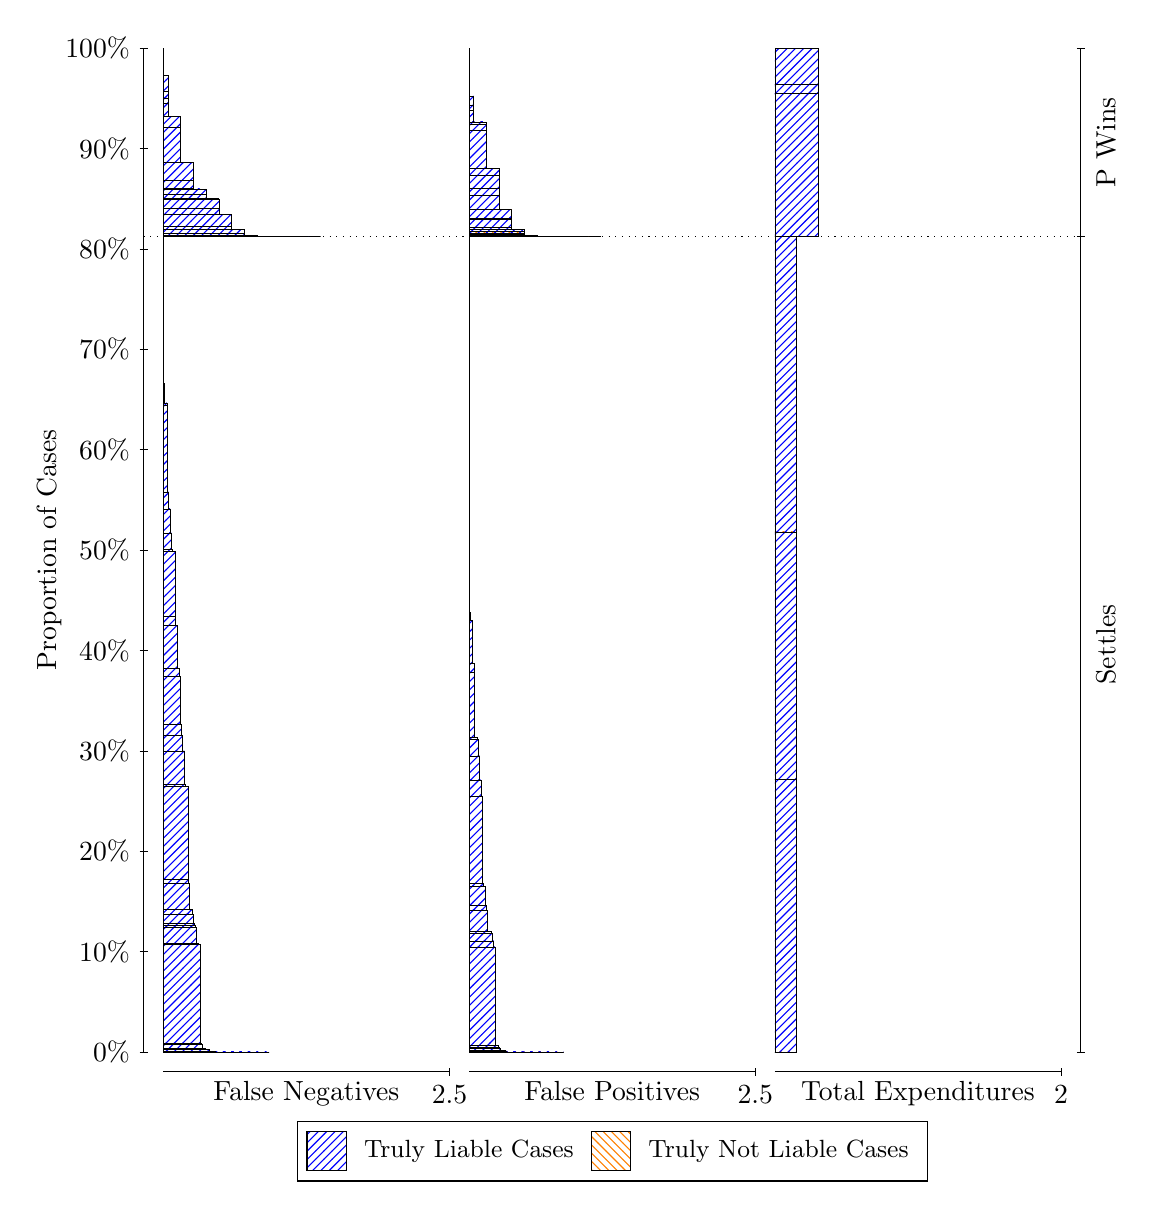
\begin{tikzpicture}
\draw[black, very thin] (1.5,1.75) -- (1.5,14.5);
\node[rotate=90, text=black, anchor=center] at (0.3, 8.125) {Proportion of Cases};
\draw[black, very thin] (1.45,1.75) -- (1.55,1.75);
\node[text=black, anchor=east] at (1.45, 1.75) {0\%};
\draw[black, very thin] (1.45,3.025) -- (1.55,3.025);
\node[text=black, anchor=east] at (1.45, 3.025) {10\%};
\draw[black, very thin] (1.45,4.3) -- (1.55,4.3);
\node[text=black, anchor=east] at (1.45, 4.3) {20\%};
\draw[black, very thin] (1.45,5.575) -- (1.55,5.575);
\node[text=black, anchor=east] at (1.45, 5.575) {30\%};
\draw[black, very thin] (1.45,6.85) -- (1.55,6.85);
\node[text=black, anchor=east] at (1.45, 6.85) {40\%};
\draw[black, very thin] (1.45,8.125) -- (1.55,8.125);
\node[text=black, anchor=east] at (1.45, 8.125) {50\%};
\draw[black, very thin] (1.45,9.4) -- (1.55,9.4);
\node[text=black, anchor=east] at (1.45, 9.4) {60\%};
\draw[black, very thin] (1.45,10.675) -- (1.55,10.675);
\node[text=black, anchor=east] at (1.45, 10.675) {70\%};
\draw[black, very thin] (1.45,11.95) -- (1.55,11.95);
\node[text=black, anchor=east] at (1.45, 11.95) {80\%};
\draw[black, very thin] (1.45,13.225) -- (1.55,13.225);
\node[text=black, anchor=east] at (1.45, 13.225) {90\%};
\draw[black, very thin] (1.45,14.5) -- (1.55,14.5);
\node[text=black, anchor=east] at (1.45, 14.5) {100\%};

\draw[black, very thin] (13.4,1.75) -- (13.4,14.5);
\draw[black, very thin] (13.35,1.75) -- (13.45,1.75);
\node[anchor=west] at (13.35, 1.75) {};
\draw[black, very thin] (13.35,12.104) -- (13.45,12.104);
\node[anchor=west] at (13.35, 12.104) {};
\draw[black, very thin] (13.35,14.5) -- (13.45,14.5);
\node[anchor=west] at (13.35, 14.5) {};

\draw[black, very thin, pattern color=blue, pattern=north east lines] (1.75,1.75) rectangle (3.0943,1.75);
\draw[black, very thin, pattern color=blue, pattern=north east lines] (1.75,1.75) rectangle (2.949,1.75);
\draw[black, very thin, pattern color=blue, pattern=north east lines] (1.75,1.75) rectangle (2.9329,1.75);
\draw[black, very thin, pattern color=blue, pattern=north east lines] (1.75,1.75) rectangle (2.8763,1.75);
\draw[black, very thin, pattern color=blue, pattern=north east lines] (1.75,1.75) rectangle (2.8037,1.75);
\draw[black, very thin, pattern color=blue, pattern=north east lines] (1.75,1.75) rectangle (2.7875,1.75);
\draw[black, very thin, pattern color=blue, pattern=north east lines] (1.75,1.75) rectangle (2.7714,1.75);
\draw[black, very thin, pattern color=blue, pattern=north east lines] (1.75,1.75) rectangle (2.731,1.75);
\draw[black, very thin, pattern color=blue, pattern=north east lines] (1.75,1.75) rectangle (2.7149,1.75);
\draw[black, very thin, pattern color=blue, pattern=north east lines] (1.75,1.75) rectangle (2.6583,1.75);
\draw[black, very thin, pattern color=blue, pattern=north east lines] (1.75,1.75) rectangle (2.6422,1.75);
\draw[black, very thin, pattern color=blue, pattern=north east lines] (1.75,1.75) rectangle (2.626,1.75);
\draw[black, very thin, pattern color=blue, pattern=north east lines] (1.75,1.75) rectangle (2.6099,1.75);
\draw[black, very thin, pattern color=blue, pattern=north east lines] (1.75,1.75) rectangle (2.5695,1.75);
\draw[black, very thin, pattern color=blue, pattern=north east lines] (1.75,1.75) rectangle (2.5534,1.75);
\draw[black, very thin, pattern color=blue, pattern=north east lines] (1.75,1.75) rectangle (2.513,1.75);
\draw[black, very thin, pattern color=blue, pattern=north east lines] (1.75,1.75) rectangle (2.4969,1.7506);
\draw[black, very thin, pattern color=blue, pattern=north east lines] (1.75,1.7506) rectangle (2.4807,1.7506);
\draw[black, very thin, pattern color=blue, pattern=north east lines] (1.75,1.7506) rectangle (2.4646,1.7506);
\draw[black, very thin, pattern color=blue, pattern=north east lines] (1.75,1.7506) rectangle (2.4484,1.7507);
\draw[black, very thin, pattern color=blue, pattern=north east lines] (1.75,1.7507) rectangle (2.4403,1.7511);
\draw[black, very thin, pattern color=blue, pattern=north east lines] (1.75,1.7511) rectangle (2.408,1.7536);
\draw[black, very thin, pattern color=blue, pattern=north east lines] (1.75,1.7536) rectangle (2.3919,1.7538);
\draw[black, very thin, pattern color=blue, pattern=north east lines] (1.75,1.7538) rectangle (2.3515,1.7541);
\draw[black, very thin, pattern color=blue, pattern=north east lines] (1.75,1.7541) rectangle (2.3354,1.7782);
\draw[black, very thin, pattern color=blue, pattern=north east lines] (1.75,1.7782) rectangle (2.3192,1.7787);
\draw[black, very thin, pattern color=blue, pattern=north east lines] (1.75,1.7787) rectangle (2.3031,1.7792);
\draw[black, very thin, pattern color=blue, pattern=north east lines] (1.75,1.7792) rectangle (2.2869,1.7849);
\draw[black, very thin, pattern color=blue, pattern=north east lines] (1.75,1.7849) rectangle (2.2789,1.7924);
\draw[black, very thin, pattern color=blue, pattern=north east lines] (1.75,1.7924) rectangle (2.2466,1.8506);
\draw[black, very thin, pattern color=blue, pattern=north east lines] (1.75,1.8506) rectangle (2.2304,1.8575);
\draw[black, very thin, pattern color=blue, pattern=north east lines] (1.75,1.8575) rectangle (2.2223,3.1206);
\draw[black, very thin, pattern color=blue, pattern=north east lines] (1.75,3.1206) rectangle (2.19,3.1261);
\draw[black, very thin, pattern color=blue, pattern=north east lines] (1.75,3.1261) rectangle (2.1739,3.3375);
\draw[black, very thin, pattern color=blue, pattern=north east lines] (1.75,3.3375) rectangle (2.1577,3.3609);
\draw[black, very thin, pattern color=blue, pattern=north east lines] (1.75,3.3609) rectangle (2.1416,3.3815);
\draw[black, very thin, pattern color=blue, pattern=north east lines] (1.75,3.3815) rectangle (2.1254,3.5027);
\draw[black, very thin, pattern color=blue, pattern=north east lines] (1.75,3.5027) rectangle (2.1174,3.5563);
\draw[black, very thin, pattern color=blue, pattern=north east lines] (1.75,3.5563) rectangle (2.0851,3.8903);
\draw[black, very thin, pattern color=blue, pattern=north east lines] (1.75,3.8903) rectangle (2.0689,3.9486);
\draw[black, very thin, pattern color=blue, pattern=north east lines] (1.75,3.9486) rectangle (2.0609,5.1245);
\draw[black, very thin, pattern color=blue, pattern=north east lines] (1.75,5.1245) rectangle (2.0286,5.1507);
\draw[black, very thin, pattern color=blue, pattern=north east lines] (1.75,5.1507) rectangle (2.0124,5.5742);
\draw[black, very thin, pattern color=blue, pattern=north east lines] (1.75,5.5742) rectangle (1.9963,5.7667);
\draw[black, very thin, pattern color=blue, pattern=north east lines] (1.75,5.7667) rectangle (1.9801,5.9173);
\draw[black, very thin, pattern color=blue, pattern=north east lines] (1.75,5.9173) rectangle (1.964,6.5235);
\draw[black, very thin, pattern color=blue, pattern=north east lines] (1.75,6.5235) rectangle (1.9559,6.6186);
\draw[black, very thin, pattern color=blue, pattern=north east lines] (1.75,6.6186) rectangle (1.9236,7.1644);
\draw[black, very thin, pattern color=blue, pattern=north east lines] (1.75,7.1644) rectangle (1.9074,7.2856);
\draw[black, very thin, pattern color=blue, pattern=north east lines] (1.75,7.2856) rectangle (1.8994,8.1057);
\draw[black, very thin, pattern color=blue, pattern=north east lines] (1.75,8.1057) rectangle (1.8671,8.1314);
\draw[black, very thin, pattern color=blue, pattern=north east lines] (1.75,8.1314) rectangle (1.8509,8.3432);
\draw[black, very thin, pattern color=blue, pattern=north east lines] (1.75,8.3432) rectangle (1.8348,8.6483);
\draw[black, very thin, pattern color=blue, pattern=north east lines] (1.75,8.6483) rectangle (1.8186,8.8621);
\draw[black, very thin, pattern color=blue, pattern=north east lines] (1.75,8.8621) rectangle (1.8025,9.9611);
\draw[black, very thin, pattern color=blue, pattern=north east lines] (1.75,9.9611) rectangle (1.7944,9.9937);
\draw[black, very thin, pattern color=blue, pattern=north east lines] (1.75,9.9937) rectangle (1.7621,10.239);
\draw[black, very thin, pattern color=orange, pattern=north west lines] (1.75,10.239) rectangle (1.75,10.239);
\draw[black, very thin, pattern color=blue, pattern=north east lines] (1.75,10.239) rectangle (1.75,12.104);
\draw[black, very thin, pattern color=blue, pattern=north east lines] (1.75,12.104) rectangle (3.7483,12.104);
\draw[black, very thin, pattern color=blue, pattern=north east lines] (1.75,12.104) rectangle (3.5869,12.104);
\draw[black, very thin, pattern color=blue, pattern=north east lines] (1.75,12.104) rectangle (3.4254,12.104);
\draw[black, very thin, pattern color=blue, pattern=north east lines] (1.75,12.104) rectangle (3.2639,12.104);
\draw[black, very thin, pattern color=blue, pattern=north east lines] (1.75,12.104) rectangle (3.2639,12.104);
\draw[black, very thin, pattern color=blue, pattern=north east lines] (1.75,12.104) rectangle (3.1024,12.106);
\draw[black, very thin, pattern color=blue, pattern=north east lines] (1.75,12.106) rectangle (3.0984,12.106);
\draw[black, very thin, pattern color=blue, pattern=north east lines] (1.75,12.106) rectangle (2.9409,12.121);
\draw[black, very thin, pattern color=blue, pattern=north east lines] (1.75,12.121) rectangle (2.9369,12.121);
\draw[black, very thin, pattern color=blue, pattern=north east lines] (1.75,12.121) rectangle (2.7794,12.15);
\draw[black, very thin, pattern color=blue, pattern=north east lines] (1.75,12.15) rectangle (2.7794,12.195);
\draw[black, very thin, pattern color=blue, pattern=north east lines] (1.75,12.195) rectangle (2.7754,12.195);
\draw[black, very thin, pattern color=blue, pattern=north east lines] (1.75,12.195) rectangle (2.7754,12.195);
\draw[black, very thin, pattern color=blue, pattern=north east lines] (1.75,12.195) rectangle (2.618,12.238);
\draw[black, very thin, pattern color=blue, pattern=north east lines] (1.75,12.238) rectangle (2.618,12.389);
\draw[black, very thin, pattern color=blue, pattern=north east lines] (1.75,12.389) rectangle (2.6139,12.39);
\draw[black, very thin, pattern color=blue, pattern=north east lines] (1.75,12.39) rectangle (2.4565,12.462);
\draw[black, very thin, pattern color=blue, pattern=north east lines] (1.75,12.462) rectangle (2.4565,12.583);
\draw[black, very thin, pattern color=blue, pattern=north east lines] (1.75,12.583) rectangle (2.4524,12.584);
\draw[black, very thin, pattern color=blue, pattern=north east lines] (1.75,12.584) rectangle (2.4524,12.589);
\draw[black, very thin, pattern color=blue, pattern=north east lines] (1.75,12.589) rectangle (2.295,12.645);
\draw[black, very thin, pattern color=blue, pattern=north east lines] (1.75,12.645) rectangle (2.291,12.712);
\draw[black, very thin, pattern color=blue, pattern=north east lines] (1.75,12.712) rectangle (2.1335,12.717);
\draw[black, very thin, pattern color=blue, pattern=north east lines] (1.75,12.717) rectangle (2.1295,12.815);
\draw[black, very thin, pattern color=blue, pattern=north east lines] (1.75,12.815) rectangle (2.1295,13.043);
\draw[black, very thin, pattern color=blue, pattern=north east lines] (1.75,13.043) rectangle (1.972,13.043);
\draw[black, very thin, pattern color=blue, pattern=north east lines] (1.75,13.043) rectangle (1.968,13.489);
\draw[black, very thin, pattern color=blue, pattern=north east lines] (1.75,13.489) rectangle (1.968,13.636);
\draw[black, very thin, pattern color=blue, pattern=north east lines] (1.75,13.636) rectangle (1.8106,13.636);
\draw[black, very thin, pattern color=blue, pattern=north east lines] (1.75,13.636) rectangle (1.8065,13.802);
\draw[black, very thin, pattern color=blue, pattern=north east lines] (1.75,13.802) rectangle (1.8065,13.867);
\draw[black, very thin, pattern color=blue, pattern=north east lines] (1.75,13.867) rectangle (1.8065,13.949);
\draw[black, very thin, pattern color=blue, pattern=north east lines] (1.75,13.949) rectangle (1.8065,14.151);
\draw[black, very thin, pattern color=orange, pattern=north west lines] (1.75,14.151) rectangle (1.75,14.151);
\draw[black, very thin, pattern color=blue, pattern=north east lines] (1.75,14.151) rectangle (1.75,14.5);
\draw[black, very thin, pattern color=orange, pattern=north west lines] (5.6333,1.75) rectangle (6.8323,1.75);
\draw[black, very thin, pattern color=blue, pattern=north east lines] (5.6333,1.75) rectangle (6.8323,1.75);
\draw[black, very thin, pattern color=blue, pattern=north east lines] (5.6333,1.75) rectangle (6.6709,1.75);
\draw[black, very thin, pattern color=orange, pattern=north west lines] (5.6333,1.75) rectangle (6.6143,1.75);
\draw[black, very thin, pattern color=blue, pattern=north east lines] (5.6333,1.75) rectangle (6.6143,1.75);
\draw[black, very thin, pattern color=orange, pattern=north west lines] (5.6333,1.75) rectangle (6.5417,1.75);
\draw[black, very thin, pattern color=blue, pattern=north east lines] (5.6333,1.75) rectangle (6.5417,1.75);
\draw[black, very thin, pattern color=blue, pattern=north east lines] (5.6333,1.75) rectangle (6.5094,1.75);
\draw[black, very thin, pattern color=blue, pattern=north east lines] (5.6333,1.75) rectangle (6.4529,1.75);
\draw[black, very thin, pattern color=orange, pattern=north west lines] (5.6333,1.75) rectangle (6.3963,1.75);
\draw[black, very thin, pattern color=blue, pattern=north east lines] (5.6333,1.75) rectangle (6.3963,1.75);
\draw[black, very thin, pattern color=blue, pattern=north east lines] (5.6333,1.75) rectangle (6.3802,1.75);
\draw[black, very thin, pattern color=blue, pattern=north east lines] (5.6333,1.75) rectangle (6.3479,1.75);
\draw[black, very thin, pattern color=orange, pattern=north west lines] (5.6333,1.75) rectangle (6.3237,1.75);
\draw[black, very thin, pattern color=blue, pattern=north east lines] (5.6333,1.75) rectangle (6.3237,1.75);
\draw[black, very thin, pattern color=blue, pattern=north east lines] (5.6333,1.75) rectangle (6.2914,1.75);
\draw[black, very thin, pattern color=orange, pattern=north west lines] (5.6333,1.75) rectangle (6.251,1.75);
\draw[black, very thin, pattern color=blue, pattern=north east lines] (5.6333,1.75) rectangle (6.251,1.7501);
\draw[black, very thin, pattern color=blue, pattern=north east lines] (5.6333,1.7501) rectangle (6.2349,1.7501);
\draw[black, very thin, pattern color=blue, pattern=north east lines] (5.6333,1.7501) rectangle (6.2187,1.7501);
\draw[black, very thin, pattern color=blue, pattern=north east lines] (5.6333,1.7501) rectangle (6.1864,1.7506);
\draw[black, very thin, pattern color=orange, pattern=north west lines] (5.6333,1.7506) rectangle (6.1783,1.7506);
\draw[black, very thin, pattern color=blue, pattern=north east lines] (5.6333,1.7506) rectangle (6.1783,1.7511);
\draw[black, very thin, pattern color=blue, pattern=north east lines] (5.6333,1.7511) rectangle (6.1622,1.7517);
\draw[black, very thin, pattern color=blue, pattern=north east lines] (5.6333,1.7517) rectangle (6.1299,1.7517);
\draw[black, very thin, pattern color=orange, pattern=north west lines] (5.6333,1.7517) rectangle (6.1057,1.7517);
\draw[black, very thin, pattern color=blue, pattern=north east lines] (5.6333,1.7517) rectangle (6.1057,1.7626);
\draw[black, very thin, pattern color=blue, pattern=north east lines] (5.6333,1.7626) rectangle (6.0895,1.7685);
\draw[black, very thin, pattern color=blue, pattern=north east lines] (5.6333,1.7685) rectangle (6.0734,1.769);
\draw[black, very thin, pattern color=blue, pattern=north east lines] (5.6333,1.769) rectangle (6.0572,1.7692);
\draw[black, very thin, pattern color=blue, pattern=north east lines] (5.6333,1.7692) rectangle (6.0249,1.7955);
\draw[black, very thin, pattern color=blue, pattern=north east lines] (5.6333,1.7955) rectangle (6.0169,1.8034);
\draw[black, very thin, pattern color=blue, pattern=north east lines] (5.6333,1.8034) rectangle (6.0007,1.8294);
\draw[black, very thin, pattern color=blue, pattern=north east lines] (5.6333,1.8294) rectangle (5.9684,1.8314);
\draw[black, very thin, pattern color=orange, pattern=north west lines] (5.6333,1.8314) rectangle (5.9603,1.8314);
\draw[black, very thin, pattern color=blue, pattern=north east lines] (5.6333,1.8314) rectangle (5.9603,3.0836);
\draw[black, very thin, pattern color=blue, pattern=north east lines] (5.6333,3.0836) rectangle (5.9442,3.1604);
\draw[black, very thin, pattern color=blue, pattern=north east lines] (5.6333,3.1604) rectangle (5.928,3.2548);
\draw[black, very thin, pattern color=blue, pattern=north east lines] (5.6333,3.2548) rectangle (5.9119,3.2787);
\draw[black, very thin, pattern color=blue, pattern=north east lines] (5.6333,3.2787) rectangle (5.8957,3.2836);
\draw[black, very thin, pattern color=blue, pattern=north east lines] (5.6333,3.2836) rectangle (5.8634,3.5555);
\draw[black, very thin, pattern color=blue, pattern=north east lines] (5.6333,3.5555) rectangle (5.8554,3.6146);
\draw[black, very thin, pattern color=blue, pattern=north east lines] (5.6333,3.6146) rectangle (5.8392,3.8602);
\draw[black, very thin, pattern color=blue, pattern=north east lines] (5.6333,3.8602) rectangle (5.8069,3.8929);
\draw[black, very thin, pattern color=blue, pattern=north east lines] (5.6333,3.8929) rectangle (5.7989,4.9918);
\draw[black, very thin, pattern color=blue, pattern=north east lines] (5.6333,4.9918) rectangle (5.7827,5.2057);
\draw[black, very thin, pattern color=blue, pattern=north east lines] (5.6333,5.2057) rectangle (5.7666,5.5108);
\draw[black, very thin, pattern color=blue, pattern=north east lines] (5.6333,5.5108) rectangle (5.7504,5.7225);
\draw[black, very thin, pattern color=blue, pattern=north east lines] (5.6333,5.7225) rectangle (5.7343,5.7483);
\draw[black, very thin, pattern color=blue, pattern=north east lines] (5.6333,5.7483) rectangle (5.702,6.5683);
\draw[black, very thin, pattern color=blue, pattern=north east lines] (5.6333,6.5683) rectangle (5.6939,6.6896);
\draw[black, very thin, pattern color=blue, pattern=north east lines] (5.6333,6.6896) rectangle (5.6777,7.2354);
\draw[black, very thin, pattern color=blue, pattern=north east lines] (5.6333,7.2354) rectangle (5.6454,7.3304);
\draw[black, very thin, pattern color=blue, pattern=north east lines] (5.6333,7.3304) rectangle (5.6374,7.9366);
\draw[black, very thin, pattern color=blue, pattern=north east lines] (5.6333,7.9366) rectangle (5.6333,12.104);
\draw[black, very thin, pattern color=orange, pattern=north west lines] (5.6333,12.104) rectangle (7.3047,12.104);
\draw[black, very thin, pattern color=blue, pattern=north east lines] (5.6333,12.104) rectangle (7.3047,12.104);
\draw[black, very thin, pattern color=orange, pattern=north west lines] (5.6333,12.104) rectangle (7.1432,12.104);
\draw[black, very thin, pattern color=blue, pattern=north east lines] (5.6333,12.104) rectangle (7.1432,12.104);
\draw[black, very thin, pattern color=orange, pattern=north west lines] (5.6333,12.104) rectangle (6.9817,12.104);
\draw[black, very thin, pattern color=blue, pattern=north east lines] (5.6333,12.104) rectangle (6.9817,12.104);
\draw[black, very thin, pattern color=blue, pattern=north east lines] (5.6333,12.104) rectangle (6.9817,12.104);
\draw[black, very thin, pattern color=blue, pattern=north east lines] (5.6333,12.104) rectangle (6.9817,12.104);
\draw[black, very thin, pattern color=orange, pattern=north west lines] (5.6333,12.104) rectangle (6.8202,12.104);
\draw[black, very thin, pattern color=blue, pattern=north east lines] (5.6333,12.104) rectangle (6.8202,12.104);
\draw[black, very thin, pattern color=blue, pattern=north east lines] (5.6333,12.104) rectangle (6.8202,12.104);
\draw[black, very thin, pattern color=orange, pattern=north west lines] (5.6333,12.104) rectangle (6.6587,12.104);
\draw[black, very thin, pattern color=blue, pattern=north east lines] (5.6333,12.104) rectangle (6.6587,12.104);
\draw[black, very thin, pattern color=blue, pattern=north east lines] (5.6333,12.104) rectangle (6.6587,12.105);
\draw[black, very thin, pattern color=blue, pattern=north east lines] (5.6333,12.105) rectangle (6.4973,12.109);
\draw[black, very thin, pattern color=orange, pattern=north west lines] (5.6333,12.109) rectangle (6.4973,12.109);
\draw[black, very thin, pattern color=blue, pattern=north east lines] (5.6333,12.109) rectangle (6.4973,12.111);
\draw[black, very thin, pattern color=blue, pattern=north east lines] (5.6333,12.111) rectangle (6.4973,12.117);
\draw[black, very thin, pattern color=blue, pattern=north east lines] (5.6333,12.117) rectangle (6.3358,12.136);
\draw[black, very thin, pattern color=blue, pattern=north east lines] (5.6333,12.136) rectangle (6.3358,12.152);
\draw[black, very thin, pattern color=orange, pattern=north west lines] (5.6333,12.152) rectangle (6.3358,12.152);
\draw[black, very thin, pattern color=blue, pattern=north east lines] (5.6333,12.152) rectangle (6.3358,12.176);
\draw[black, very thin, pattern color=blue, pattern=north east lines] (5.6333,12.176) rectangle (6.3358,12.192);
\draw[black, very thin, pattern color=blue, pattern=north east lines] (5.6333,12.192) rectangle (6.1743,12.226);
\draw[black, very thin, pattern color=orange, pattern=north west lines] (5.6333,12.226) rectangle (6.1743,12.226);
\draw[black, very thin, pattern color=blue, pattern=north east lines] (5.6333,12.226) rectangle (6.1743,12.33);
\draw[black, very thin, pattern color=blue, pattern=north east lines] (5.6333,12.33) rectangle (6.1743,12.342);
\draw[black, very thin, pattern color=blue, pattern=north east lines] (5.6333,12.342) rectangle (6.1743,12.453);
\draw[black, very thin, pattern color=orange, pattern=north west lines] (5.6333,12.453) rectangle (6.1703,12.453);
\draw[black, very thin, pattern color=blue, pattern=north east lines] (5.6333,12.453) rectangle (6.1703,12.453);
\draw[black, very thin, pattern color=blue, pattern=north east lines] (5.6333,12.453) rectangle (6.0128,12.632);
\draw[black, very thin, pattern color=blue, pattern=north east lines] (5.6333,12.632) rectangle (6.0128,12.718);
\draw[black, very thin, pattern color=blue, pattern=north east lines] (5.6333,12.718) rectangle (6.0128,12.886);
\draw[black, very thin, pattern color=blue, pattern=north east lines] (5.6333,12.886) rectangle (6.0128,12.968);
\draw[black, very thin, pattern color=blue, pattern=north east lines] (5.6333,12.968) rectangle (6.0088,12.968);
\draw[black, very thin, pattern color=orange, pattern=north west lines] (5.6333,12.968) rectangle (6.0088,12.968);
\draw[black, very thin, pattern color=blue, pattern=north east lines] (5.6333,12.968) rectangle (6.0088,12.968);
\draw[black, very thin, pattern color=blue, pattern=north east lines] (5.6333,12.968) rectangle (5.8513,13.456);
\draw[black, very thin, pattern color=blue, pattern=north east lines] (5.6333,13.456) rectangle (5.8513,13.528);
\draw[black, very thin, pattern color=blue, pattern=north east lines] (5.6333,13.528) rectangle (5.8513,13.561);
\draw[black, very thin, pattern color=blue, pattern=north east lines] (5.6333,13.561) rectangle (5.8473,13.561);
\draw[black, very thin, pattern color=orange, pattern=north west lines] (5.6333,13.561) rectangle (5.8473,13.561);
\draw[black, very thin, pattern color=blue, pattern=north east lines] (5.6333,13.561) rectangle (5.8473,13.561);
\draw[black, very thin, pattern color=blue, pattern=north east lines] (5.6333,13.561) rectangle (5.8473,13.561);
\draw[black, very thin, pattern color=blue, pattern=north east lines] (5.6333,13.561) rectangle (5.6899,13.714);
\draw[black, very thin, pattern color=blue, pattern=north east lines] (5.6333,13.714) rectangle (5.6899,13.772);
\draw[black, very thin, pattern color=blue, pattern=north east lines] (5.6333,13.772) rectangle (5.6899,13.883);
\draw[black, very thin, pattern color=blue, pattern=north east lines] (5.6333,13.883) rectangle (5.6899,13.887);
\draw[black, very thin, pattern color=blue, pattern=north east lines] (5.6333,13.887) rectangle (5.6858,13.888);
\draw[black, very thin, pattern color=orange, pattern=north west lines] (5.6333,13.888) rectangle (5.6858,13.888);
\draw[black, very thin, pattern color=blue, pattern=north east lines] (5.6333,13.888) rectangle (5.6858,13.891);
\draw[black, very thin, pattern color=blue, pattern=north east lines] (5.6333,13.891) rectangle (5.6858,13.892);
\draw[black, very thin, pattern color=orange, pattern=north west lines] (5.6333,13.892) rectangle (5.6333,13.892);
\draw[black, very thin, pattern color=blue, pattern=north east lines] (5.6333,13.892) rectangle (5.6333,14.5);
\draw[black, very thin, pattern color=orange, pattern=north west lines] (9.5167,1.75) rectangle (9.7892,1.75);
\draw[black, very thin, pattern color=blue, pattern=north east lines] (9.5167,1.75) rectangle (9.7892,5.2078);
\draw[black, very thin, pattern color=orange, pattern=north west lines] (9.5167,5.2078) rectangle (9.7892,5.2078);
\draw[black, very thin, pattern color=blue, pattern=north east lines] (9.5167,5.2078) rectangle (9.7892,8.355);
\draw[black, very thin, pattern color=orange, pattern=north west lines] (9.5167,8.355) rectangle (9.7892,8.355);
\draw[black, very thin, pattern color=blue, pattern=north east lines] (9.5167,8.355) rectangle (9.7892,12.104);
\draw[black, very thin, pattern color=orange, pattern=north west lines] (9.5167,12.104) rectangle (10.062,12.104);
\draw[black, very thin, pattern color=blue, pattern=north east lines] (9.5167,12.104) rectangle (10.062,13.928);
\draw[black, very thin, pattern color=orange, pattern=north west lines] (9.5167,13.928) rectangle (10.062,13.928);
\draw[black, very thin, pattern color=blue, pattern=north east lines] (9.5167,13.928) rectangle (10.062,14.041);
\draw[black, very thin, pattern color=orange, pattern=north west lines] (9.5167,14.041) rectangle (10.062,14.041);
\draw[black, very thin, pattern color=blue, pattern=north east lines] (9.5167,14.041) rectangle (10.062,14.5);
\draw[black, dotted] (1.5,12.104) -- (13.4,12.104);
\draw[black, very thin] (1.75,1.5) -- (5.3833,1.5);
\node[text=black, anchor=north] at (3.5667, 1.5) {False Negatives};
\draw[black, very thin] (5.3833,1.45) -- (5.3833,1.55);
\node[text=black, anchor=north] at (5.3833, 1.45) {2.5};

\draw[black, very thin] (5.6333,1.5) -- (9.2667,1.5);
\node[text=black, anchor=north] at (7.45, 1.5) {False Positives};
\draw[black, very thin] (9.2667,1.45) -- (9.2667,1.55);
\node[text=black, anchor=north] at (9.2667, 1.45) {2.5};

\draw[black, very thin] (9.5167,1.5) -- (13.15,1.5);
\node[text=black, anchor=north] at (11.333, 1.5) {Total Expenditures};
\draw[black, very thin] (13.15,1.45) -- (13.15,1.55);
\node[text=black, anchor=north] at (13.15, 1.45) {2};

\node[text=black, centered, rotate=90] at (13.72, 6.927) {Settles};
\node[text=black, centered, rotate=90] at (13.72, 13.302) {P Wins};

\draw (7.449999999999999,1.5) node[draw=none] (baseCoordinate) {};
\begin{scope}[align=center]
        \matrix[scale=0.5, draw=black, below=0.5cm of baseCoordinate, nodes={draw}, column sep=0.1cm]{
            \node[rectangle, draw, minimum width=0.5cm, minimum height=0.5cm, pattern color=blue, pattern=north east lines] {}; &
            \node[draw=none, font=\small, text=black] (B) {Truly Liable Cases}; &
            \node[rectangle, draw, minimum width=0.5cm, minimum height=0.5cm, pattern color=orange, pattern=north west lines] {}; &
            \node[draw=none, font=\small, text=black] (B) {Truly Not Liable Cases}; \\
            };
\end{scope}

\end{tikzpicture}
\end{document}